Im Folgenden sind die während des Versuchs aufgenommenen Messwerte tabellarisch und 
durch Grafiken dargestellt. An entsprechender Stelle sind Anmerkungen und Erklärungen zu
den Messwerten und den vollzogenen Rechnungen gegeben.  


\subsection{Messung der Zeitkonstante durch Entladung des\\ Kondensators}
	
	Die in \cref{tab:Auswertung_Entladen} gelisteten Messwerte sind aus dem in \cref{fig:Auswertung_Entladen}
	dargestellten zeitlichen Verlauf der Kondensatorspannung $ U_{C}(t) $ entnommen.
	
	\begin{figure}[!h]
		\centering
		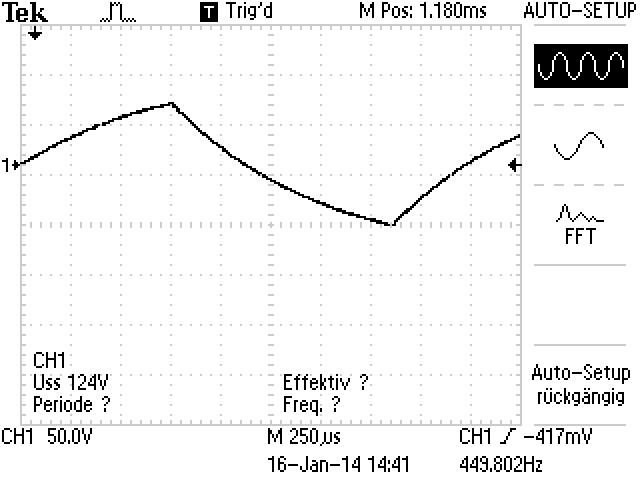
\includegraphics[scale=1]{Grafiken/Entladen.jpg}
		\caption{Zeitlicher Verlauf der Kondensatorspannung bei Entladung}
		\label{fig:Auswertung_Entladen}
	\end{figure}
    \begin{table}[!h]
	\centering
	\begin{tabular}{|c|c||c|c|}
		\hline
		Zeit & Kondensatorspannung & Zeit & Kondensatorspannung \\
		$t\,[\si{\milli\second}]$ & ${U_{C}}\,[\si{\volt}]$ & 
		$t\,[\si{\milli\second}]$ & ${U_{C}}\,[\si{\volt}]$\\\hline\hline
		\num{0.0}  & \num{121(1)} & \num{0.5}  & \num{44(1)} \\
		\num{0.1}  & \num{102(1)} & \num{0.6}  & \num{34(1)} \\
		\num{0.2}  & \num{84(1)} &  \num{0.7}  & \num{25(1)} \\
		\num{0.3}  & \num{68(1)} &  \num{0.8}  & \num{17(1)} \\
		\num{0.4}  & \num{56(1)} &  &\\
		\hline
	\end{tabular}
	\caption{Kondensatorspannung zur Zeit $t$ nach Beginn der Entladung \label{tab:Auswertung_Entladen}}
\end{table}
	
	Durch Regression der in \cref{fig:Auswertung_EntladungLog} halb-logarithmisch
	aufgetragenen Messwerte, unter Verwendung der Python Bibliothek \emph{SciPy} \cite{SciPy}, ergeben sich 
	die Parameter $ a $ und $ b $ der angesetzten Regressionsfunktion
	\begin{empheq}{equation}
		f(t) = at + b
	\end{empheq}
	zu
	\addtocounter{equation}{-1}
	\begin{subequations}
		\begin{empheq}{align}
		\label{eq:Auswertung_Entladung_Steigung}
			a &= \SI{-2127(84)}{\per\second} \\
		\label{eq:Auswertung_Entladung_Achsenabschnitt}
			b &= \SI{125(3)}{}.
		\end{empheq}		
	\end{subequations}
	
	\begin{figure}[!h]
		\centering
		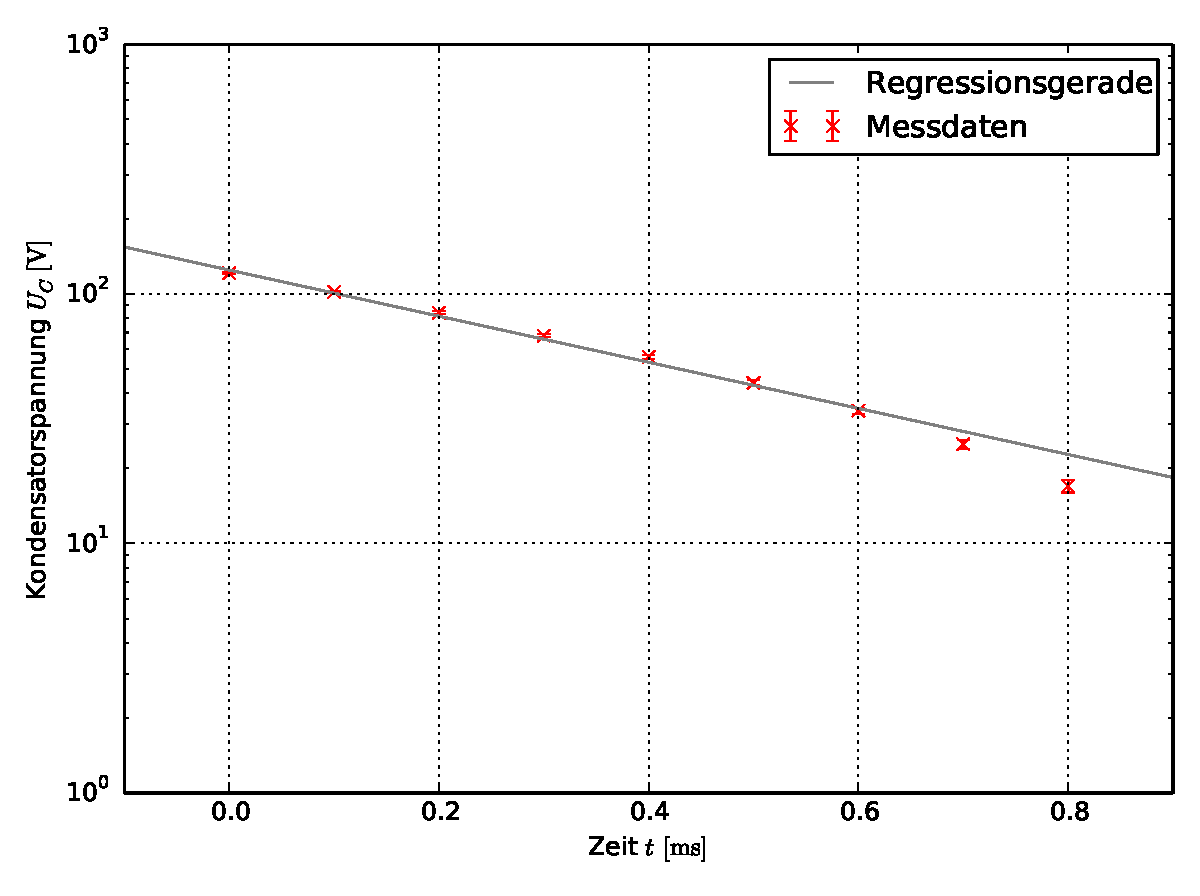
\includegraphics[scale=0.75]{Grafiken/Entladung.pdf}
		\caption{Messwerte des Entladungsvorgangs mit entsprechender Regressionsgeraden}
		\label{fig:Auswertung_EntladungLog}
	\end{figure}
	 
	Mit der theoretischen Form dieser Regressionsgeraden 
	\begin{empheq}{equation}
		\ln\del{\dfrac{U(t)}{U(0)}}  = -\dfrac{t}{RC}, 
	\end{empheq}
	die man durch logarithmieren von \cref{eq:Theorie_Entladung}
	\footnote{Da $ U = qE $ gilt sind zeitlicher Verlauf von Spannung und Ladung äquivalent} erhält
	lässt sich zeigen, dass die reziproke Steigung dieser Geraden der Zeitkonstante $ RC $  entspricht.
	Diese hat, mit der Steigung \cref{eq:Auswertung_Entladung_Steigung} somit den Wert
	\begin{empheq}{equation}
		 RC =  \dfrac{1}{a} = \SI{4.7(2)e-04}{\second}
	\end{empheq}
	 
	 
	 
\subsection{Messung der Frequenzabhängigkeit der \\ Kondensatorspannungsamplitude}

	In \cref{tab:Auswertung_Amplitude} sind die, in Abhängigkeit der Frequenz $ f_{G} $ der angelegten 
	Sinusspannung gemessenen, Amplituden der Kondensatorspannung $A(f)$ und die mit $ U_{0} = \SI{80}{\volt} $
	normierten Amplituden $ \tfrac{A(f)}{U_{0}} $ eingetragen. 
	
	\begin{table}[!h]
	\centering
	\begin{tabular}{|r|c|c|}
		\hline
		Frequenz & Amplitude & normierte Amplitude\\
		$f\,[\si{\hertz}]$ & $A(f)\,[\si{\volt}]$ & $\tfrac{A(f)}{U_{0}}$\\\hline\hline
		\num{30}  & \num{75.2(1)}  & \num{0.940(1)} \\
		\num{50}  & \num{75.0(1)}  & \num{0.938(1)} \\
		\num{70}  & \num{74.4(1)}  & \num{0.930(1)} \\
		\num{90}  & \num{71.2(1)}  & \num{0.890(1)} \\
		\num{100}  & \num{70.0(1)}  & \num{0.875(1)} \\
		\num{300}  & \num{44.0(1)}  & \num{0.550(1)} \\
		\num{500}  & \num{30.0(1)}  & \num{0.375(1)} \\
		\num{700}  & \num{22.0(1)}  & \num{0.275(1)} \\
		\num{900}  & \num{17.4(1)}  & \num{0.217(1)} \\
		\num{1000}  & \num{15.8(1)}  & \num{0.198(1)} \\
		\num{3000}  & \num{5.6(1)}  & \num{0.070(1)} \\
		\num{5000}  & \num{3.4(1)}  & \num{0.042(1)} \\
		\num{7000}  & \num{2.6(1)}  & \num{0.033(1)} \\
		\num{9000}  & \num{1.78(1)}  & \num{0.0222(1)} \\
		\num{10000}  & \num{1.62(1)}  & \num{0.0203(1)} \\
		\num{30000}  & \num{0.56(1)}  & \num{0.0070(1)} \\
		\num{50000}  & \num{0.33(1)}  & \num{0.0041(1)} \\
		\num{70000}  & \num{0.24(1)}  & \num{0.0030(1)} \\
		\num{100000}  & \num{0.17(1)}  & \num{0.0021(1)} \\
		\hline
	\end{tabular}
	\caption{Amplitude und normierte Amplitude der Kondensatorspannung in\\\hspace*{1.9cm} Abhängigkeit der Frequenz \label{tab:Auswertung_Amplitude}}
\end{table}
	
	In \cref{fig:Auswertung_Amplitude} sind die normierten Amplituden gegen die Frequenzen halb-logarithmisch 
	aufgetragen. 
	
	\begin{figure}[!h]
		\centering
		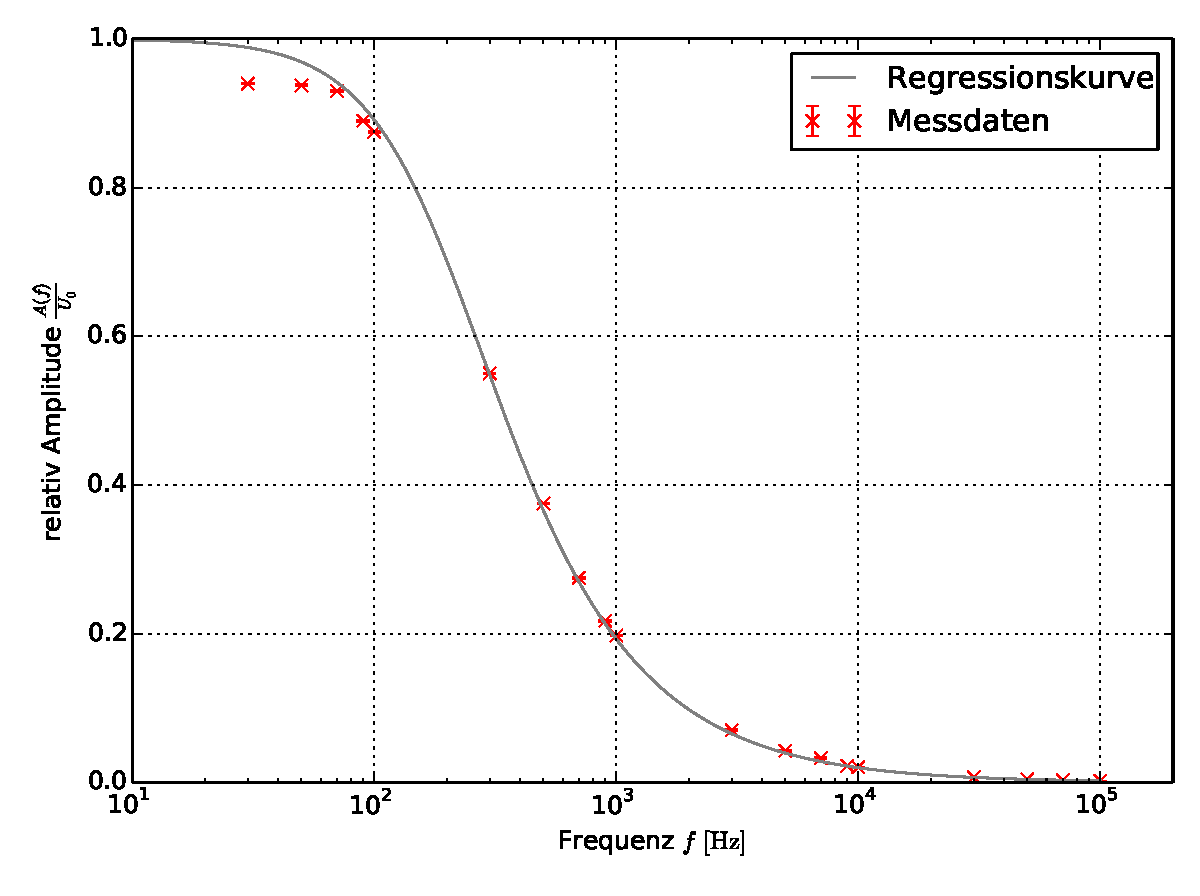
\includegraphics[scale=0.75]{Grafiken/Amplitude.pdf}
		\caption{Normierte Amplituden in Abhängigkeit von der Frequenz mit\\\hspace*{2.6cm} entsprechender Regressionskurve}
		\label{fig:Auswertung_Amplitude}
	\end{figure}
	
	Durch Regression der Messwerte für die normierte Amplitude in \cref{fig:Auswertung_Amplitude} mit eine Funktion der Form
	\begin{empheq}{equation}
		A(f) = \dfrac{1}{\sqrt{1 + c^{2} (2\pi f)^{2}}},
	\end{empheq} 
	ergibt sich der Regressionsparameter zu
	\addtocounter{equation}{-1}
	\begin{subequations}
		\begin{empheq}{equation}
		\label{eq:Auswertung_Amplitude_Param}
			c = \SI{8.1(2)e-04}{\second}
		\end{empheq} 
	\end{subequations}
	
	Der theoretische Verlauf der Amplitude in Abhängigkeit der Frequenz \cref{eq:Theorie_Amplitude} zeigt,
	dass mit \cref{eq:Auswertung_Amplitude_Param} für die Zeitkonstante $ RC $ des RC-Gliedes  
		\begin{empheq}{equation}
			RC = c = \SI{8.1(2)e-04}{\second}
		\end{empheq}	
	gilt.
	
\subsection{Messung der Frequenzabhängigkeit der Phasendifferenz\\ zwischen Generator- und Kondensatorspannung}

	Die in Abhängigkeit von der Frequenz aufgenommenen Messwerte für die Phasendifferenz zwischen Generator-
	und Kondensatorspannung $ U_{G}(t)\ \text{bzw.}\ U_{C}(t) $ sind in \cref{tab:Auswertung_Phasendifferenz}
	zu finden.
	
	\begin{table}[!h]
	\centering
	\begin{tabular}{|c|c||c|c|}
		\hline
		     Frequenz      &       Phasendifferenz        &      Frequenz      &       Phasendifferenz        \\
		$f\,[\si{\hertz}]$ & $\varphi(f)\,[\si{\degree}]$ & $f\,[\si{\hertz}]$ & $\varphi(f)\,[\si{\degree}]$ \\ \hline\hline
		    \num{100}      &         \num{18.0}         &    \num{10000}     &         \num{90.0}         \\
		    \num{200}      &         \num{54.0}         &    \num{20000}     &         \num{86.4}         \\
		    \num{300}      &         \num{64.8}         &    \num{30000}     &         \num{86.4}         \\
		    \num{400}      &         \num{57.6}         &    \num{40000}     &         \num{86.4}         \\
		    \num{500}      &         \num{63.0}         &    \num{50000}     &         \num{90.0}         \\
		    \num{1000}     &         \num{81.0}         &    \num{100000}    &         \num{90.0}         \\
		    \num{2000}     &         \num{86.4}         &    \num{200000}    &         \num{93.6}         \\
		    \num{3000}     &         \num{86.4}         &    \num{300000}    &         \num{97.2}         \\
		    \num{4000}     &         \num{93.6}         &    \num{400000}    &        \num{100.8}         \\
		    \num{5000}     &         \num{90.0}         &    \num{500000}    &         \num{90.0}         \\ \hline
	\end{tabular}
	\caption{Phasendifferenz der Kondensator- und Generatorspannung in\\\hspace*{1.9cm} Abhängigkeit der Frequenz \label{tab:Auswertung_Phasendifferenz}}
\end{table}
	\begin{figure}[!h]
		\centering
		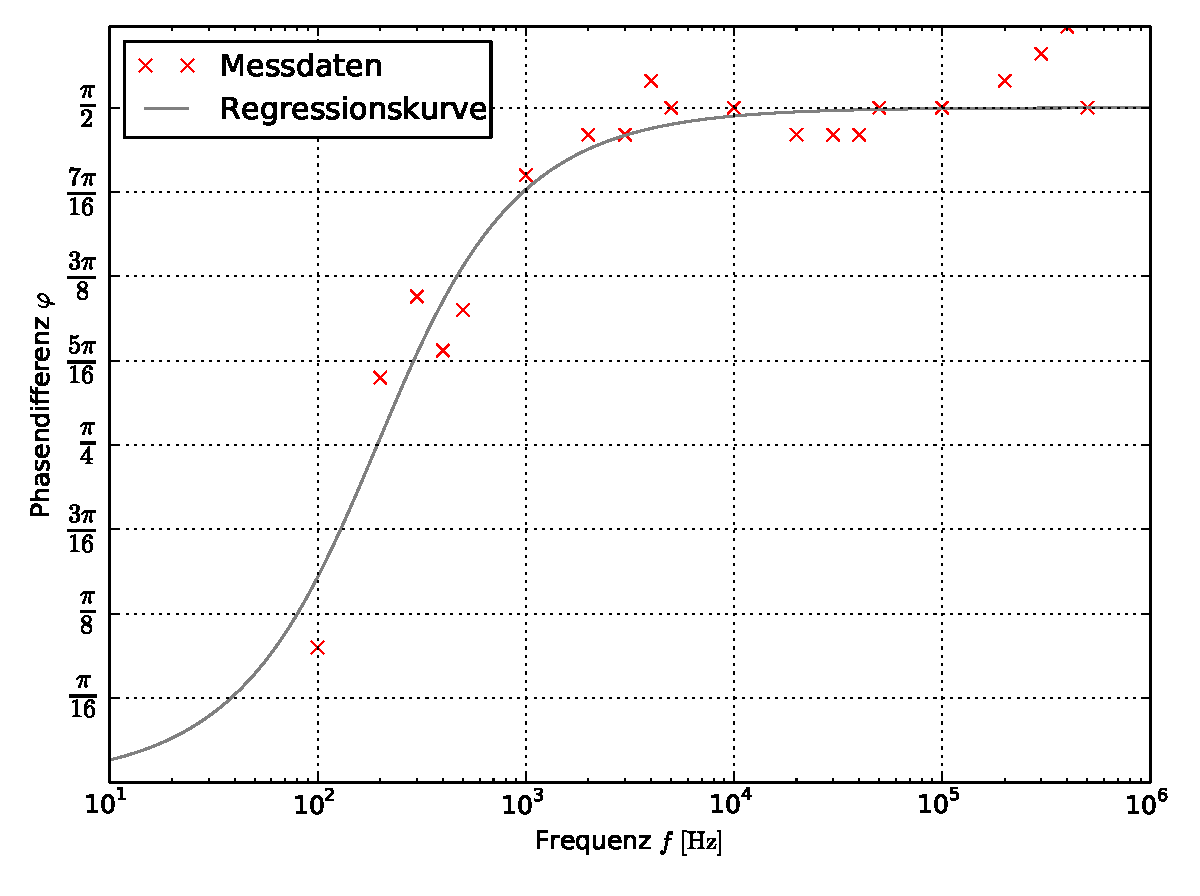
\includegraphics[scale=0.75]{Grafiken/Phasendifferenz.pdf}
		\caption{Phasendifferenz in Abhängigkeit der Frequenz mit entsprechender Regressionskurve}
		\label{fig:Auswertung_Phasendifferenz}
	\end{figure}
	
	Die mit einer Funktion der Form
	\begin{empheq}{equation}
		\varphi(f) = \arctan(d\cdot 2\pi f)
	\end{empheq}
	durchgeführte Regression der in \cref{fig:Auswertung_Phasendifferenz} dargestellten Messwerte
	liefert den Regressionsparameter
	\addtocounter{equation}{-1}
 	\begin{subequations}
		\begin{empheq}{equation}
			d =\SI{8.2(8)e-04}{\second}.
		\end{empheq}
 	\end{subequations}
	
	Aus diesem lässt sich wiederum, durch Vergleich mit dem theoretischen Verlauf der Phasendifferenz 
	\cref{eq:Theorie_Phasendiffernez} die Zeitkonstante $ RC $ des RC-Gliedes zu
		\begin{empheq}{equation}
			RC = d =\SI{8.2(8)e-04}{\second}.
		\end{empheq}
	
	
	
\subsection{Darstellung der Kondensatorspannungsamplitude in\\ Abhängigkeit der Frequenz und der Phasendifferenz }

	Durch das Einsetzten der Gleichungen für die Frequenzabhängigkeit der Amplitude und Phasendifferenz 
	\cref{eq:Theorie_Amplitude} bzw. \cref{eq:Theorie_Phasendiffernz} in \cref{eq:Theorie_Amplitude_Phase}
	ergibt sich der Zusammenhang zwischen normierter Amplitude und Phasendifferenz zu:
	\begin{empheq}{align}
		\dfrac{A(\omega)}{U_{0}} &= -\dfrac{\sin(\arctan(-\omega RC))}{\omega RC} \nonumber\\
		 &= \dfrac{\sin(\arctan(\omega RC))}{\omega RC} \nonumber\\
		 &= \dfrac{\omega RC}{\sqrt{1 + (\omega RC)^{2}} \omega RC} \nonumber\\
		 &= \dfrac{1}{\sqrt{1 + (\omega RC)^{2}}} \nonumber\\
		 &= \cos(\arctan(-\omega RC)) \nonumber\\
		 \label{eq:Auswertung_Amplitude_Phase}
		\dfrac{A(\omega)}{U_{0}} &= \cos(\varphi(\omega))  
	\end{empheq}
	 
	Mit dieser Gleichung erhält man den in \cref{fig:Auswertung_Amplitude_Phase} dargestellten Verlauf.
	Die ebenso eingezeichneten Messwerte sind \cref{tab:Auswertung_Amplitude} und 
	\ref{tab:Auswertung_Phasendifferenz} entnommen.
	
	\begin{figure}[!h]
		\centering
		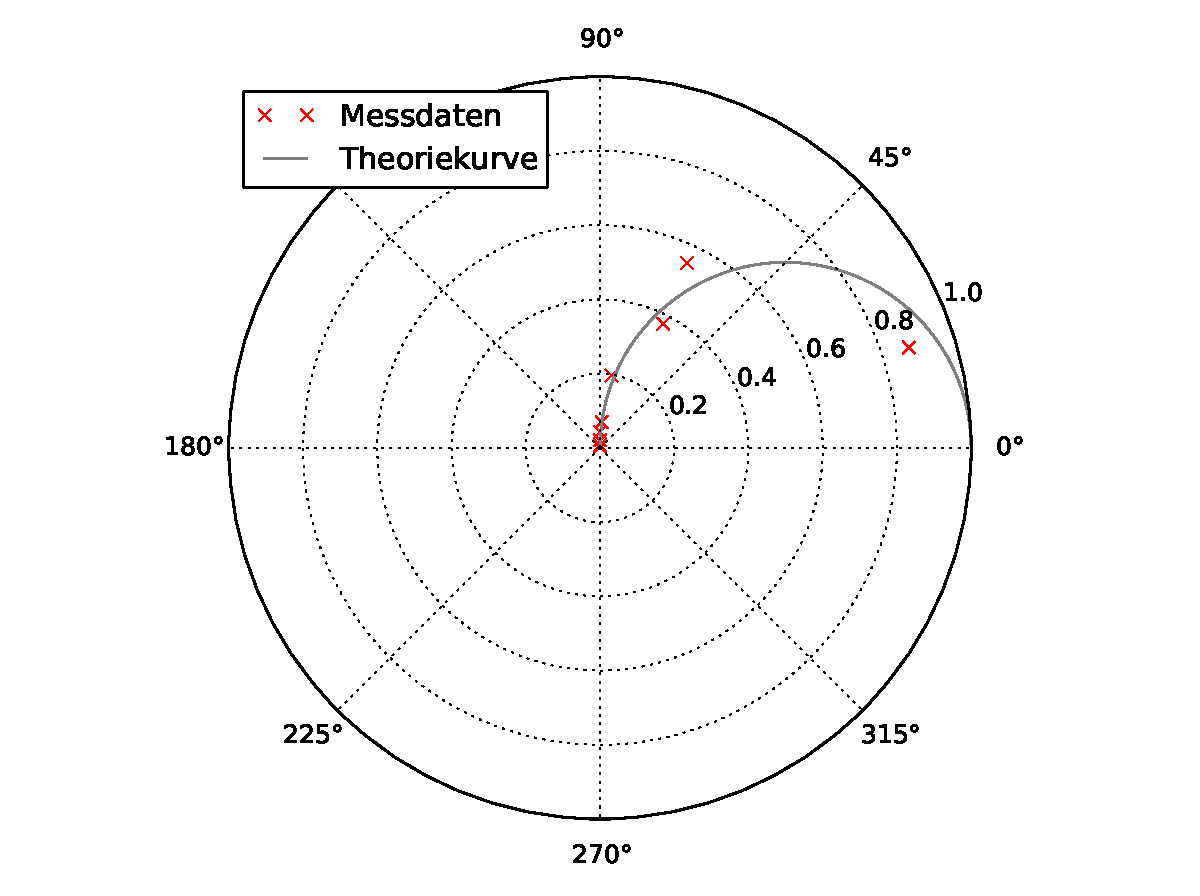
\includegraphics[scale=0.5]{Grafiken/Amplitude_Polar.pdf}
		\caption{Verlauf der normierten Amplitude in Abhängigkeit von der Phasendifferenz}
		\label{fig:Auswertung_Amplitude_Phase}
	\end{figure}
	 
\subsection{Das RC-Glied als Integrator}
	
	In den folgenden Abbildungen sind die aufgenommen Spannungsverläufe der Sinus-, Dreieck- und Rechteckspannung
	und dem jeweiligen Spannungsverlauf $U_{C}$ der Kondensatorspannung dargestellt.
	
	\begin{figure}[!h]
		\centering
		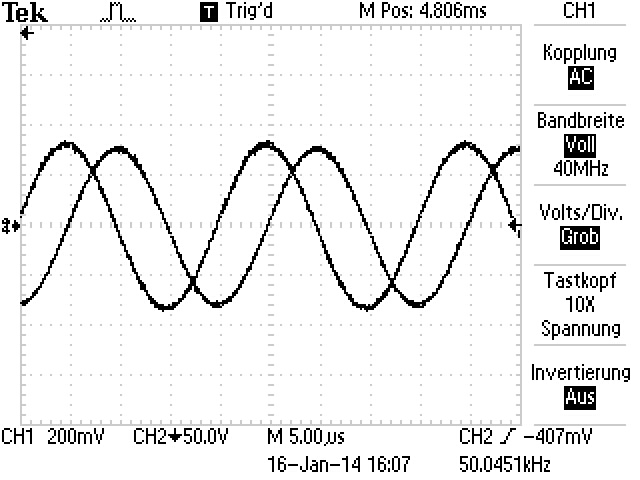
\includegraphics[scale=0.7]{Grafiken/Integrator_Sinus.jpg}
		\caption{Integration des Sinusspannung}
		\label{fig:Auswertung_Integrator_Sinus}
	\end{figure}
	
	\begin{figure}[!h]
		\centering
		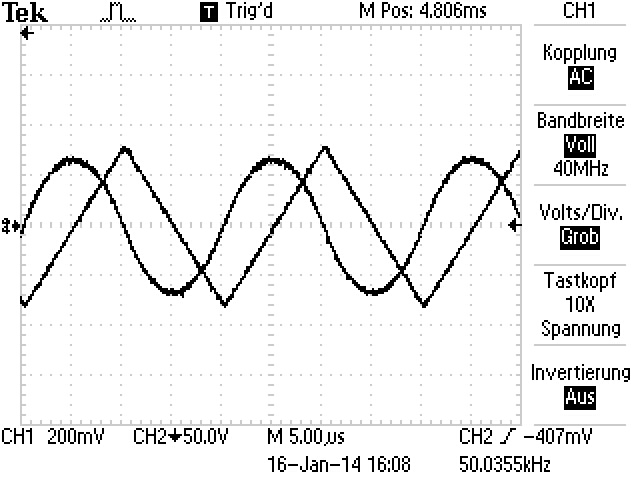
\includegraphics[scale=0.7]{Grafiken/Integrator_Dreieck.jpg}
		\caption{Integration des Dreieckspannung}
		\label{fig:Auswertung_Integrator_Dreieck}
	\end{figure}
	
	\begin{figure}[!h]
		\centering
		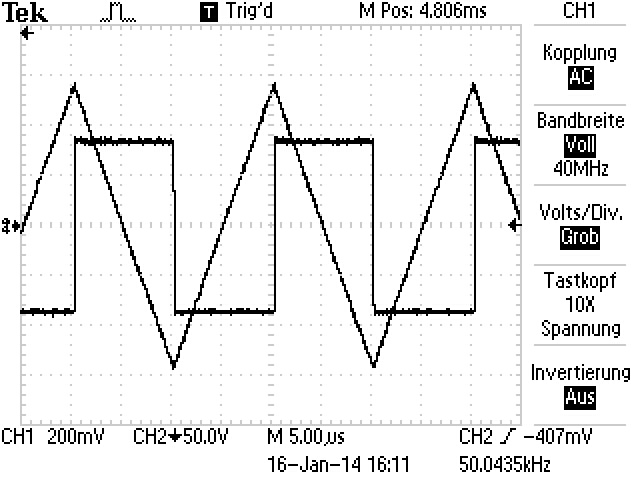
\includegraphics[scale=0.7]{Grafiken/Integrator_Rechteck.jpg}
		\caption{Integration der Rechteckspannung}
		\label{fig:Auswertung_Integrator_Rechteck}
	\end{figure}